\documentclass[12pt]{article}

\usepackage[T1]{fontenc}
\usepackage{graphicx}
\graphicspath{ {./images/} } 
\usepackage{float}
\begin{document}

(Q)
Describe: ...
\clearpage

Challenges of Distributed Systems\\
SCC311\\
\begin{figure}[H]

\includegraphics[width=0.5\linewidth]{page1-image-1.png}
\end{figure}
\clearpage
(Q)
Describe: Overview of the Session
\clearpage
\section{Overview of the Session}
\\
\begin{itemize}
  \item Two Generals problem
  \item Byzantine Generals problem
  \item Fallacies of distributed computing
  \item Middleware
\end{itemize}
\clearpage
(Q)
Describe: Two Generals Problem
\clearpage
\section{Two Generals Problem}
\\
\end{itemize}
  \item  Complication in distributed consensus
\begin{itemize}
  \item  Two generals, each leading an army, want to capture a city. The 
\end{itemize}
attack is only successful if both armies attack together\\
\begin{itemize}
  \item  Coordination is vital
  \item  Generals need to reach consensus in order
\end{itemize}
to succeed in conquering the city.\\
Belisarius\\
Narses\\
City\\
General1 General2\\
messengers\\
Attack or notAttack or not\\
\begin{figure}[H]

\includegraphics[width=0.5\linewidth]{page3-image-1.png}
\end{figure}
\begin{figure}[H]

\includegraphics[width=0.5\linewidth]{page3-image-2.png}
\end{figure}
\begin{figure}[H]

\includegraphics[width=0.5\linewidth]{page3-image-3.png}
\end{figure}
\clearpage
(Q)
Describe: Two Generals Problem
\clearpage
\section{Two Generals Problem}
\\
\begin{itemize}
  \item  Complication in distributed consensus
\begin{itemize}
  \item  Two generals, each leading an army, want to capture a city. The 
\end{itemize}
\end{itemize}
attack is only successful if both armies attack together\\
Belisarius\\
Narses\\
City\\
General1 General2\\
messengers\\
Attack or notAttack or not\\
Army1 Army2 Result\\
No Attack No attack Nothing happens\\
No Attack Attack Army2 defeated\\
Attack No attack Army1 defeated\\
Attack Attack City captured\\
\begin{figure}[H]

\includegraphics[width=0.5\linewidth]{page4-image-1.png}
\end{figure}
\begin{figure}[H]

\includegraphics[width=0.5\linewidth]{page4-image-2.png}
\end{figure}
\begin{figure}[H]

\includegraphics[width=0.5\linewidth]{page4-image-3.png}
\end{figure}
\clearpage
(Q)
Describe: Two Generals Problem
\clearpage
\section{Two Generals Problem}
\\
\begin{itemize}
  \item  Important challenges
\begin{itemize}
  \item  Faulty network
  \item  Receipt of Acknowledgement is necessary
\end{itemize}
\end{itemize}
General1 General2\\
Attack on Oct 14 ?\\
Acknowledged!\\
General1 General2\\
Attack on Oct 14 ?\\
time time time time\\
\clearpage
(Q)
Describe: How the generals should 
\clearpage
\section{How the generals should }
\\
decide?\\
\begin{itemize}
  \item  Is it possible to come up with an algorithm that works all the time ? 
  \item  Answer is no.
  \item  Possible approaches (none of them fully works): 
  \item  Approach 1
  \item  General1 sends a lot of messages at once, and then attacks
  \item  Problem: if all the messengers are captured, army1 is defeated
  \item  Approach 2
  \item  General1 attacks only if an ACK is received from General 2
  \item  Now general2 will be captured if its response is intercepted or delayed
  \item  Problem: General2 has no idea if his ACK is received by General1
  \item  In the two generals problem, we assume a faulty network but processes 
\end{itemize}
(i.e., generals) are not faulty. \\
\clearpage
(Q)
Describe: FLP Impossibility Result
\clearpage
\section{FLP Impossibility Result}
\\
\begin{itemize}
  \item  FLP impossibility result
  \item  Fischer, Lynch, and Patterson, Impossibility of Distributed Consensus with One Faulty 
\end{itemize}
Process, 1985\\
\begin{itemize}
  \item  Asynchronous systems:
  \item  No bounds on message delivery time and process execution time
  \item  Clock drifts are also unbounded
  \item  When there is no upper bound on the time a process takes to complete its work and 
\end{itemize}
respond, it’s impossible to make the distinction between a process that is crashed and one \\
that is working (but taking very long to respond). \\
\begin{itemize}
  \item  FLP shows that there is no guarantee for distributed processes to reach consensus in an 
\end{itemize}
asynchronous environment, where it’s possible for at least one process to crash. \\
\begin{itemize}
  \item  Equivalently, it’s not always possible to detect failure in an asynchronous system with 
\end{itemize}
nodes crashing.\\
\begin{itemize}
  \item  So let’s consider the case where messages are delivered reliably (i.e., network is 
\end{itemize}
not faulty) next. \\
\clearpage
(Q)
Describe: Byzantine Generals Problem
\clearpage
\section{Byzantine Generals Problem}
\\
We imagine that several divisions of the Byzantine army are \\
camped outside an enemy city, each division has its own general. \\
One commanding general (on behalf of the emperor) sends an \\
order to the lieutenant generals. However, some of the generals, \\
including the commanding general, may be traitors. The generals \\
must have an algorithm to guarantee that:\\
\begin{itemize}
  \item All loyal lieutenant generals decide upon the same plan of 
\end{itemize}
action. \\
\begin{itemize}
  \item A small number of traitors cannot cause the loyal generals to 
\end{itemize}
adopt a bad plan.” \\
L. Lamport, R. Shostak, and M. Pease, “The Byzantine Generals Problem”, 1982 \\
\clearpage
(Q)
Describe: Byzantine Generals Problem
\clearpage
\section{Byzantine Generals Problem}
\\
The Byzantine Generals Problem \\
LESLIE LAMPORT, ROBERT SHOSTAK, and MARSHALL PEASE \\
SRI International \\
Re lia ble  compute r sys tems  mus t ha ndle  ma lfunctioning compone nts  tha t give  conflicting informa tion \\
to diffe rent pa rts  of the  sys tem. This  s itua tion ca n be  expressed a bs tra ctly in te rms  of a  group of \\
genera ls  of the  Byza ntine  a rmy ca mpe d with the ir troops  a round a n e ne my city. Communica ting only \\
by messenger, the  genera ls  mus t agree  upon a  common ba ttle  pla n. However, one  or more  of the m \\
ma y be  tra itors  who will try to confuse  the  others . The  proble m is  to find a n a lgorithm to e ns ure  tha t \\
the  loya l genera ls  will re a ch agreement. It is  shown tha t, us ing only ora l messages , this  proble m is  \\
solvable  if a nd only if more  tha n two-thirds  of the  genera ls  a re  loya l; so a  s ingle  tra itor ca n confound \\
two loya l genera ls . With unforgeable  writte n messages , the  proble m is  solvable  for a ny numbe r of \\
genera ls  a nd poss ible  tra itors . Applica tions  of the  s olutions  to re lia ble  compute r s ys te ms  a re  the n \\
discussed. \\
Ca tegories  a nd S ubje ct Descriptors : C.2.4. [C o m p u te r-C o m m u n ic a tio n  Ne tworks ]: Dis tribute d \\
S ys tems--ne twork operating systems; D.4.4 [O p e ra tin g  S ys te ms ]: Communica tions  Ma na ge me nt-- \\
network communication; D.4.5 [O p e ra tin g  S ys te ms ]: Reliability--fault tolerance  \\
Ge ne ra l Te rms : Algorithms, Re lia bility \\
Additiona l Ke y Words  a nd Phrases : Inte ra ctive  cons is tency \\
/ \\
1 . INTR O DUC TIO N \\
A re lia b le  c o m p u t e r  s y s t e m  m u s t  b e  a b le  to  c o p e  with  th e  fa ilu re  o f o n e  o r m o re  \\
o f its  c o m p o n e n t s .  A fa ile d  c o m p o n e n t  m a y  e xh ib it  a  typ e  o f b e h a v io r  t h a t  is  \\
o ft e n  o v e r lo o k e d - - n a m e ly ,  s e n d in g  c o n flic t in g  in fo r m a t io n  to  d iffe re n t  p a r t s  o f \\
t h e  s ys te m .  T h e  p r o b le m  o f c o p in g  with  th is  typ e  o f fa ilu re  is  e xp re s s e d  a b s t r a c t ly  \\
a s  th e  B y z a n t in e  G e n e r a ls  P ro b le m .  W e  d e vo te  th e  m a jo r  p a r t  o f th e  p a p e r  to  a  \\
d is c u s s io n  o f th is  a b s t r a c t  p r o b le m  a n d  c o n c lu d e  b y  in d ic a t in g  h o w o u r  s o lu t io n s  \\
c a n  b e  u s e d  in  im p le m e n t in g  a  re lia b le  c o m p u t e r  s ys te m .  \\
W e  im a g in e  t h a t  s e ve ra l d iv is io n s  o f th e  B y z a n t in e  a r m y  a re  c a m p e d  o u ts id e  \\
a n  e n e m y  c ity,  e a c h  d iv is io n  c o m m a n d e d  b y  its  o w n  g e n e ra l.  T h e  g e n e ra ls  c a n  \\
c o m m u n ic a t e  with  o n e  a n o t h e r  o n ly  b y  m e s s e n g e r .  Afte r  o b s e rv in g  th e  e n e m y ,  \\
t h e y  m u s t  d e c id e  u p o n  a  c o m m o n  p la n  o f a c t io n .  Ho we ve r ,  s o m e  o f th e  g e n e ra ls  \\
This  research was  s upporte d in  pa rt by the  Na tiona l Ae rona utics  a nd Space  Adminis tra tion unde r \\
contra ct NAS1-15428 Mod. 3, the  Ballis tic Miss ile  Defense  S ys te ms  Comma nd unde r contra ct \\
DASG60-78-C-0046, a nd the  Army Research Office  unde r contra ct DAAG29-79-C-0102. \\
Authors ' address : Compute r Science  Labora tory, S RI Inte rna tiona l, 333 Ravenswood Avenue , Me nlo \\
P a rk, CA 94025. \\
P e rmis s ion to copy without fee  a ll or pa rt of this  ma te ria l is  gra nte d provided tha t the  copies  a re  not \\
ma de  or dis tribute d for dire ct commercia l advantage , the  ACM copyright notice  a nd the  title  of the  \\
publica tion a nd its  da te  appear, a nd notice  is  given tha t copying is  by permiss ion of the  Associa tion \\
for Computing Machinery. To copy otherwise , or to republish, requires  a  fee  a nd/or specific \\
permiss ion. \\
© 1982 ACM 0164-0925/82/0700-0382 \$00.75 \\
ACM Transactions  on Programming Languages and Systems, Vol. 4, No. 3, July 1982, Pages 382-401. \\
\begin{figure}[H]

\includegraphics[width=0.5\linewidth]{page9-image-1.png}
\end{figure}
\clearpage
(Q)
Describe: Byzantine Generals Problem
\clearpage
\section{Byzantine Generals Problem}
\\
\begin{itemize}
  \item  3 processes, commanding general is disloyal
\end{itemize}
Lieutenant1 Lieutenant2\\
Commander\\
??\\
\begin{figure}[H]

\includegraphics[width=0.5\linewidth]{page10-image-1.png}
\end{figure}
\clearpage
(Q)
Describe: Byzantine Generals Problem
\clearpage
\section{Byzantine Generals Problem}
\\
\begin{itemize}
  \item  3 processes, commanding general is disloyal
\end{itemize}
Lieutenant1 Lieutenant2\\
Commander\\
Retreat!Attack!\\
\begin{figure}[H]

\includegraphics[width=0.5\linewidth]{page11-image-1.png}
\end{figure}
\clearpage
(Q)
Describe: Byzantine Generals Problem
\clearpage
\section{Byzantine Generals Problem}
\\
\begin{itemize}
  \item  What should the loyal lieutenants do to follow a unified course 
\end{itemize}
of action?\\
Lieutenant1 Lieutenant2\\
Commander\\
Retreat!Attack!\\
\begin{figure}[H]

\includegraphics[width=0.5\linewidth]{page12-image-1.png}
\end{figure}
\clearpage
(Q)
Describe: Byzantine Generals Problem
\clearpage
\section{Byzantine Generals Problem}
\\
\begin{itemize}
  \item  What should lieutenants do ?
  \item  Lieutenants can communicate with one another and
\end{itemize}
compare notes\\
Lieutenant1 Lieutenant2\\
Commander\\
Retreat!Attack!\\
\begin{figure}[H]

\includegraphics[width=0.5\linewidth]{page13-image-1.png}
\end{figure}
\clearpage
(Q)
Describe: Byzantine Generals Problem
\clearpage
\section{Byzantine Generals Problem}
\\
\begin{itemize}
  \item  Comparing notes (by sending messages to each other)
  \item  Remember this time network is not faulty 
\end{itemize}
Lieutenant1 Lieutenant2\\
I was told\\
Attack\\
I was told\\
Retreat\\
Commander\\
Retreat!Attack!\\
\begin{figure}[H]

\includegraphics[width=0.5\linewidth]{page14-image-1.png}
\end{figure}
\clearpage
(Q)
Describe: Byzantine Generals Problem
\clearpage
\section{Byzantine Generals Problem}
\\
\begin{itemize}
  \item  Lieutenants can’t agree on the commander’s order so they do 
\end{itemize}
the default action which is retreat.\\
Commander\\
Lieutenant1 Lieutenant2\\
Retreat!Attack!\\
I was told\\
Attack\\
I was told\\
Retreat\\
\begin{figure}[H]

\includegraphics[width=0.5\linewidth]{page15-image-1.png}
\end{figure}
\clearpage
(Q)
Describe: Byzantine Generals Problem
\clearpage
\section{Byzantine Generals Problem}
\\
\begin{itemize}
  \item  Both scenarios are equivalent from Lieutenant1’s point of view
\end{itemize}
Commander\\
Lieutenant1 Lieutenant2\\
Retreat!Attack!\\
I was \\
told\\
Attack\\
I was \\
told\\
Retreat\\
Commander\\
Lieutenant1 Lieutenant2\\
Attack!Attack!\\
I was \\
told\\
Attack\\
I was \\
told\\
Retreat\\
\begin{figure}[H]

\includegraphics[width=0.5\linewidth]{page16-image-1.png}
\end{figure}
\begin{figure}[H]

\includegraphics[width=0.5\linewidth]{page16-image-2.png}
\end{figure}
\clearpage
(Q)
Describe: Byzantine Generals Problem
\clearpage
\section{Byzantine Generals Problem}
\\
\begin{itemize}
  \item  Both scenarios are equivalent from Lieutenant2’s point of view
\end{itemize}
Commander\\
Lieutenant1 Lieutenant2\\
Retreat!Attack!\\
I was \\
told\\
Attack\\
I was \\
told\\
Retreat\\
Commander\\
Lieutenant1 Lieutenant2\\
Attack!Attack!\\
I was \\
told\\
Retreat\\
I was \\
told\\
Attack\\
\begin{figure}[H]

\includegraphics[width=0.5\linewidth]{page17-image-1.png}
\end{figure}
\begin{figure}[H]

\includegraphics[width=0.5\linewidth]{page17-image-2.png}
\end{figure}
\clearpage
(Q)
Describe: Byzantine Generals Problem
\clearpage
\section{Byzantine Generals Problem}
\\
\begin{itemize}
  \item  With d = 1 traitor, the Byzantine Generals problem is not 
\end{itemize}
solvable with 3 generals\\
\begin{itemize}
  \item  Consensus is not possible
  \item  You need at least 4 nodes! (see next slide)
\end{itemize}
Commander\\
Lieutenant1 Lieutenant2\\
Attack!Attack!\\
I was told\\
Attack\\
I was told\\
Retreat\\
\begin{figure}[H]

\includegraphics[width=0.5\linewidth]{page18-image-1.png}
\end{figure}
\clearpage
(Q)
Describe: Byzantine Generals Problem
\clearpage
\section{Byzantine Generals Problem}
\\
\begin{itemize}
  \item  With more than 3 participants, the strategy is still the same
  \item  All lieutenants compare notes with each other
  \item  Then follow the majority “vote”
  \item  If the majority was told “Attack”, then attack 
  \item  If the majority was told “Retreat!”, then retreat
\end{itemize}
Commander\\
Lieutenant1 Lieutenant2\\
Attack!Attack!\\
I was told\\
Attack\\
I was told\\
Retreat\\
\begin{figure}[H]

\includegraphics[width=0.5\linewidth]{page19-image-1.png}
\end{figure}
\clearpage
(Q)
Describe: Byzantine Generals Problem
\clearpage
\section{Byzantine Generals Problem}
\\
\begin{itemize}
  \item  Communicating notes only work with one traitor
\end{itemize}
Commander\\
Lieutenant1\\
Retreat!Attack!\\
Lieutenant2 Lieutenant3 Lieutenant4 Lieutenant5 Lieutenant6 Lieutenant7\\
\begin{figure}[H]

\includegraphics[width=0.5\linewidth]{page20-image-1.png}
\end{figure}
\begin{figure}[H]

\includegraphics[width=0.5\linewidth]{page20-image-2.png}
\end{figure}
\clearpage
(Q)
Describe: Byzantine Generals Problem
\clearpage
\section{Byzantine Generals Problem}
\\
\begin{itemize}
  \item  Let’s say all lieutenants compare notes as before
  \item  Each lieutenant sends a message to every other lieutenant and 
\end{itemize}
indicates the order it received\\
Commander\\
Lieutenant1\\
Retreat!Attack!\\
I was told\\
Attack\\
Lieutenant2 Lieutenant3 Lieutenant4 Lieutenant5 Lieutenant6 Lieutenant7\\
I was told\\
Attack\\
I was told\\
Attack\\
I was told\\
Retreat\\
I was told\\
Retreat\\
I was told\\
Retreat\\
\begin{figure}[H]

\includegraphics[width=0.5\linewidth]{page21-image-1.png}
\end{figure}
\begin{figure}[H]

\includegraphics[width=0.5\linewidth]{page21-image-2.png}
\end{figure}
\clearpage
(Q)
Describe: Byzantine Generals Problem
\clearpage
\section{Byzantine Generals Problem}
\\
\begin{itemize}
  \item  Let’s say all lieutenants compare notes as before
  \item  Each lieutenant sends a message to every other lieutenant and 
\end{itemize}
indicates the order it received\\
Commander\\
Lieutenant1\\
Retreat!Attack!\\
I was told\\
Attack\\
Lieutenant2 Lieutenant3 Lieutenant4 Lieutenant5 Lieutenant6 Lieutenant7\\
\begin{figure}[H]

\includegraphics[width=0.5\linewidth]{page22-image-1.png}
\end{figure}
\begin{figure}[H]

\includegraphics[width=0.5\linewidth]{page22-image-2.png}
\end{figure}
\clearpage
(Q)
Describe: Byzantine Generals Problem
\clearpage
\section{Byzantine Generals Problem}
\\
\begin{itemize}
  \item  How can the traitor lieutenant disrupt the majority vote and 
\end{itemize}
cause chaos ?  \\
Commander\\
Lieutenant1\\
Retreat!Attack!\\
Lieutenant2 Lieutenant3 Lieutenant4 Lieutenant5 Lieutenant6 Lieutenant7\\
Attack:3\\
Retreat: 3\\
Attack:3\\
Retreat: 3\\
Attack:3\\
Retreat: 3\\
Attack:3\\
Retreat: 3\\
Attack:3\\
Retreat: 3\\
Attack:3\\
Retreat: 3\\
\begin{figure}[H]

\includegraphics[width=0.5\linewidth]{page23-image-1.png}
\end{figure}
\begin{figure}[H]

\includegraphics[width=0.5\linewidth]{page23-image-2.png}
\end{figure}
\clearpage
(Q)
Describe: Byzantine Generals Problem
\clearpage
\section{Byzantine Generals Problem}
\\
\begin{itemize}
  \item  How can the traitor lieutenant disrupt the majority vote and 
\end{itemize}
cause chaos ?  \\
Commander\\
Lieutenant1\\
Retreat!Attack!\\
Lieutenant2 Lieutenant3 Lieutenant4 Lieutenant5 Lieutenant6 Lieutenant7\\
I was told\\
Retreat\\
I was told\\
Attack\\
\begin{figure}[H]

\includegraphics[width=0.5\linewidth]{page24-image-1.png}
\end{figure}
\begin{figure}[H]

\includegraphics[width=0.5\linewidth]{page24-image-2.png}
\end{figure}
\clearpage
(Q)
Describe: Byzantine Generals Problem
\clearpage
\section{Byzantine Generals Problem}
\\
\begin{itemize}
  \item  How can the traitor lieutenant disrupt the majority vote and 
\end{itemize}
cause chaos ?  \\
Commander\\
Lieutenant1\\
Retreat!Attack!\\
Lieutenant2 Lieutenant3 Lieutenant4 Lieutenant5 Lieutenant6 Lieutenant7\\
Attack:4\\
Retreat: 3\\
Attack:4\\
Retreat: 3\\
Attack:4\\
Retreat: 3\\
Attack:3\\
Retreat: 4\\
Attack:3\\
Retreat: 4\\
Attack:3\\
Retreat: 4\\
\begin{figure}[H]

\includegraphics[width=0.5\linewidth]{page25-image-1.png}
\end{figure}
\begin{figure}[H]

\includegraphics[width=0.5\linewidth]{page25-image-2.png}
\end{figure}
\clearpage
(Q)
Describe: Byzantine Generals Problem
\clearpage
\section{Byzantine Generals Problem}
\\
\begin{itemize}
  \item  The solution to this problem is more rounds of communication 
\end{itemize}
between lieutenants!\\
\begin{itemize}
  \item  In addition to what they heard from the commander,
\end{itemize}
lieutenants also share what they heard from each other. \\
Commander\\
Lieutenant1\\
Retreat!Attack!\\
Lieutenant2 Lieutenant3 Lieutenant4 Lieutenant5 Lieutenant6 Lieutenant7\\
L1 L2 L3 L4 L5 L6 L7\\
A A A A R R R\\
L1 L2 L3 L4 L5 L6 L7\\
R A A A R R R\\
\begin{figure}[H]

\includegraphics[width=0.5\linewidth]{page26-image-1.png}
\end{figure}
\begin{figure}[H]

\includegraphics[width=0.5\linewidth]{page26-image-2.png}
\end{figure}
\clearpage
(Q)
Describe: Byzantine Generals Problem
\clearpage
\section{Byzantine Generals Problem}
\\
\begin{itemize}
  \item  For lieutenant2:
  \item  For liutenant5: 
\end{itemize}
Commander\\
Lieutenant1\\
Retreat!Attack!\\
Lieutenant2 Lieutenant3 Lieutenant4 Lieutenant5 Lieutenant6 Lieutenant7\\
L1 L3 L4 L5 L6 L7\\
A A A R R R\\
L1 L2 L3 L4 L6 L7\\
R A A A R R\\
I was told\\
Retreat\\
I was told\\
Attack\\
\begin{figure}[H]

\includegraphics[width=0.5\linewidth]{page27-image-1.png}
\end{figure}
\begin{figure}[H]

\includegraphics[width=0.5\linewidth]{page27-image-2.png}
\end{figure}
\clearpage
(Q)
Describe: Byzantine Generals Problem
\clearpage
\section{Byzantine Generals Problem}
\\
\begin{itemize}
  \item  Then, the lieutenants exchange their vectors with each other
  \item  Each compose a table, where each row is a vector that is 
\end{itemize}
exchanged in the previous round\\
Commander\\
Lieutenant1\\
Retreat!Attack!\\
Lieutenant2 Lieutenant3 Lieutenant4 Lieutenant5 Lieutenant6 Lieutenant7\\
L1 L2 L3 L4 L5 L6 L7\\
L1 X X X X X X\\
L2 A A A R R R\\
L3 A A A R R R\\
L4 A A A R R R\\
L5 R A A A R R\\
L6 R A A A R R\\
L7 R A A A R R\\
I was told\\
Retreat\\
I was told\\
Attack\\
\begin{figure}[H]

\includegraphics[width=0.5\linewidth]{page28-image-1.png}
\end{figure}
\begin{figure}[H]

\includegraphics[width=0.5\linewidth]{page28-image-2.png}
\end{figure}
\clearpage
(Q)
Describe: Byzantine Generals Problem
\clearpage
\section{Byzantine Generals Problem}
\\
\begin{itemize}
  \item  Assumption: there is a default 
\end{itemize}
action in case loyal lieutenants can \\
not agree on an action\\
\begin{itemize}
  \item  Default = Retreat
  \item  Then, the lieutenants exchange their 
\end{itemize}
vectors with each other\\
\begin{itemize}
  \item  Lieutenant5:
\end{itemize}
L1 L2 L3 L4 L5 L6 L7\\
L1 X X X X X X\\
L2 A A A R R R\\
L3 A A A R R R\\
L4 A A A R R R\\
L5 R A A A R R\\
L6 R A A A R R\\
L7 R A A A R R\\
? A A A R R R\\
Apply majority() to each column\\
\clearpage
(Q)
Describe: Summary of Lamport’s Algorithm 
\clearpage
\section{Summary of Lamport’s Algorithm }
\\
\begin{itemize}
  \item  For d traitors, there has to be more than 3d generals
  \item  For d faulty nodes, the algorithm requires a total of d+1 rounds of 
\end{itemize}
communication (d rounds of comparing notes + order from the commander)\\
\begin{itemize}
  \item  Lamport’s algorithm provides Byzantine Fault tolerance, given that you 
\end{itemize}
have more than 3d generals (processes)\\
\begin{itemize}
  \item  Byzantine fault model: a process can behave arbitrarily (even 
\end{itemize}
maliciously as in the Byzantine Generals problem)\\
\begin{itemize}
  \item  There are other fault models such as crash-stop (i.e., a process can 
\end{itemize}
stop responding), which are less challenging to deal with than the \\
Byzantine fault model \\
\begin{itemize}
  \item  We will cover fault tolerance in detail during week 5
  \item  Can we somehow make sure lieutenants don’t forge orders that they didn’t 
\end{itemize}
receive? \\
\begin{itemize}
  \item  Public key cryptography can help with this – signed messages
  \item  However, traitors can collaborate and share their keys with each other
  \item  We will cover public key cryptography next week
\end{itemize}
\clearpage
(Q)
Describe: Applications of Byzantine 
\clearpage
\section{Applications of Byzantine }
\\
Fault Tolerance\\
\end{itemize}
  \item  Space flight
  \item  Space shuttle had 4 computers for decision making
  \item  They used a majoritarian system in case of disagreements
  \item  Cryptocurrency: there are financial incentives to act maliciously
  \item  Problems stem from having multiple control systems
\begin{itemize}
  \item  e.g. air traffic control, airline bookings, critical manufacturing 
\end{itemize}
processes, stock exchange, etc.\\
\begin{itemize}
  \item  Lamport’s algorithm is expensive! – O(n2) messaging overhead 
\end{itemize}
each round. \\
\begin{itemize}
  \item  Alternative: accept uncertainty, just work around it
\begin{itemize}
  \item  e.g. send a predetermined number of messages and assume at 
\end{itemize}
\end{itemize}
least one gets to the destination\\
\begin{itemize}
  \item  Assume at most d=1 or 2  simultaneous bad actors 
\end{itemize}
\clearpage
(Q)
Describe: Further complications
\clearpage
\section{Further complications}
\\
\begin{itemize}
  \item  Heterogeneity
\end{itemize}
  \item  Access
  \item  Platform
  \item  Format
  \item  Administration
\begin{itemize}
  \item  Changing nature
\end{itemize}
  \item  Increase/decrease in scale
  \item  Churn
  \item  Relocation
  \item  Failure
\end{itemize}
\begin{figure}[H]

\includegraphics[width=0.5\linewidth]{page32-image-1.png}
\end{figure}
\clearpage
(Q)
Describe: Fallacies of distributed computing
\clearpage
\section{Fallacies of distributed computing}
\\
\begin{itemize}
  \item  Asserted by Peter Deutsch (Sun Microsystems)
\end{itemize}
\end{itemize}
1. The network is reliable\\
2. Latency is zero\\
3. Bandwidth is infinite\\
4. The network is secure\\
5. There is one administrator\\
6. Transport cost is zero\\
7. The network is homogeneous\\
8. Topology doesn't change\\
\begin{figure}[H]

\includegraphics[width=0.5\linewidth]{page33-image-1.png}
\end{figure}
\begin{figure}[H]

\includegraphics[width=0.5\linewidth]{page33-image-2.png}
\end{figure}
\begin{figure}[H]

\includegraphics[width=0.5\linewidth]{page33-image-3.png}
\end{figure}
\begin{figure}[H]
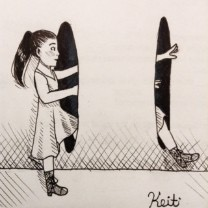
\includegraphics[width=0.5\linewidth]{page33-image-4.png}
\end{figure}
\begin{figure}[H]
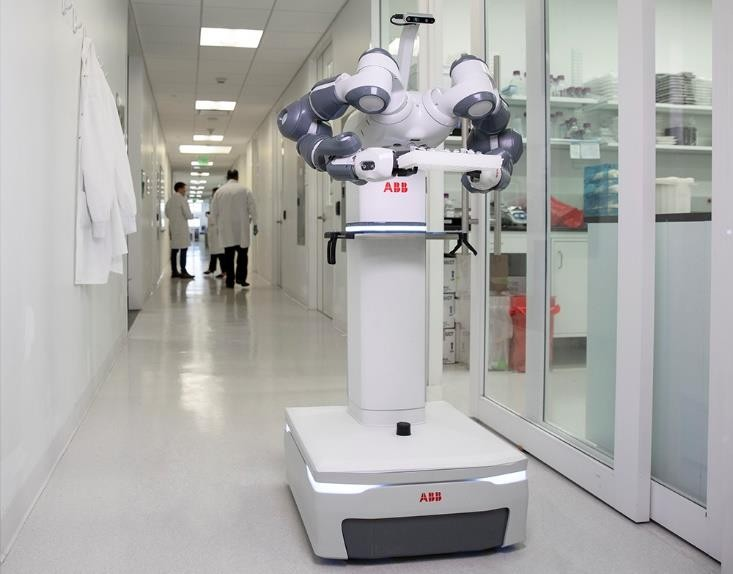
\includegraphics[width=0.5\linewidth]{page33-image-5.png}
\end{figure}
\begin{figure}[H]

\includegraphics[width=0.5\linewidth]{page33-image-6.png}
\end{figure}
\begin{figure}[H]

\includegraphics[width=0.5\linewidth]{page33-image-7.png}
\end{figure}
\begin{figure}[H]

\includegraphics[width=0.5\linewidth]{page33-image-8.png}
\end{figure}
\begin{figure}[H]

\includegraphics[width=0.5\linewidth]{page33-image-9.png}
\end{figure}
\clearpage
(Q)
Describe: The Take-away Message?
\clearpage
\section{The Take-away Message?}
\\
\begin{itemize}
  \item  Challenging
\begin{itemize}
  \item Developing good software is difficult
  \item Developing good distributed software is even harder
\end{itemize}
  \item  To do this you need help!
\begin{itemize}
  \item  Very hard to build such systems on bare-bones devices
  \item  Strong need for software platforms - \textgreater  Middleware
\end{itemize}
\begin{figure}[H]

\includegraphics[width=0.5\linewidth]{page34-image-1.png}
\end{figure}
\clearpage
(Q)
Describe: Middleware
\clearpage
\section{Middleware}
\\
\end{itemize}
  \item  Rationale
\begin{itemize}
  \item  Provide a high level programming abstraction
  \item  Hide the complexity associated with distributed systems 
\end{itemize}
\end{itemize}
(including the underlying forms of heterogeneity)\\
Machine A Machine B Machine C\\
Network\\
Network OS \\
Services\\
Middleware\\
Kernel KernelKernel\\
Network OS \\
Services\\
Network OS \\
Services\\
Distributed applications\\
uted Applic\\
\clearpage
(Q)
Describe: Goals of a Middleware Platform
\clearpage
\section{Goals of a Middleware Platform}
\\
Middleware provides protocols to support:\\
\begin{itemize}
  \item  Resource sharing
\begin{itemize}
  \item  The ability to access and share resources in a distributed environment
  \item  Distributed locking
\end{itemize}
  \item  Transparency
\begin{itemize}
  \item  The ability to view a distributed system as if it were a single computer
  \item  Varying dimensions of transparency incl. location, access, migration, etc.
\end{itemize}
  \item  Openness
\begin{itemize}
  \item  The offering of services according to standard rules (syntax and semantics)
  \item  Openness provides support for the key properties of:
\end{itemize}
\end{itemize}
0 Portability: ability to run across different platforms\\
0 Interoperability: having separate parts harmoniously work together\\
\begin{itemize}
  \item  Extensibility
\begin{itemize}
  \item  The ability to be able to introduce new or modified functionality
\end{itemize}
\clearpage
(Q)
Describe: Goals of a Middleware Platform
\clearpage
\section{Goals of a Middleware Platform}
\\
\end{itemize}
  \item  Scalability: the ability to grow/shrink with respect to
\begin{itemize}
  \item  Size
\end{itemize}
\end{itemize}
0 e.g. support massive growth in the number of users of a service\\
\begin{itemize}
  \item  Geography
\end{itemize}
0 e.g. supporting systems across continents (dealing with latencies, etc.)\\
\begin{itemize}
  \item  Administration
\end{itemize}
0 e.g. supporting systems spanning many different administrative organisations\\
\begin{itemize}
  \item  Dependability/ Quality of Service
\begin{itemize}
  \item  Security
\end{itemize}
\end{itemize}
0 Providing secure and authenticated channels, access control, key \\
management, etc.\\
\begin{itemize}
  \item  Fault tolerance
\end{itemize}
0 Providing highly available and resilient distributed applications and services\\
\clearpage
(Q)
Describe: Styles of Middleware
\clearpage
\section{Styles of Middleware}
\\
\begin{itemize}
  \item  Client-server platforms
\begin{itemize}
  \item  e.g. DCE (Distributed Computing Environment) – first!
\end{itemize}
  \item  Distributed object technology
\begin{itemize}
  \item  e.g. CORBA, Java RMI
\end{itemize}
  \item  Component-based programming
\begin{itemize}
  \item  e.g. Fractal, Enterprise Java Beans, OpenCOM
\end{itemize}
  \item  Microservice architecture
\begin{itemize}
  \item  Loosely coupled, testable services using CI/CD
\end{itemize}
  \item  Others styles
\begin{itemize}
  \item  Resource discovery platforms (e.g. Jini)
  \item  Group communication services (e.g. JGroups)
  \item  Publish-subscribe systems (e.g. JMS)
  \item  Distributed file systems, distributed transaction services, distributed
\end{itemize}
\end{itemize}
document-based systems, agent-based systems, message-oriented\\
middleware, P2P technologies, etc.\\
\clearpage
(Q)
Describe: Expected Learning Outcomes
\clearpage
\section{Expected Learning Outcomes}
\\
At the end of this session, you should:\\
\begin{itemize}
  \item  Have an intuition of why realising good distributed systems is 
\end{itemize}
difficult\\
\begin{itemize}
  \item  Byzantine generals problem as an example
\begin{itemize}
  \item  Understand what the role of middleware in supporting the 
\end{itemize}
\end{itemize}
development of distributed applications and services\\
\begin{itemize}
  \item  Goals of middleware systems
  \item  Some different styles of middleware
\end{itemize}
\clearpage
(Q)
Describe: Additional Reading
\clearpage
\section{Additional Reading}
\\
\begin{itemize}
  \item  CDKB, chapter 1 section 1.5
\end{itemize}
  \item  also chapter 3 for revision
\begin{itemize}
  \item  TvS, chapter 1, and sections 8.1-8.2
  \item  Lamport, Shostak, Pease, “The Byzantine Generals Problem”,
\end{itemize}
\end{itemize}
ACM Transactions on Programming Languages and Systems,\\
July 1982. http://dl.acm.org/citation.cfm?id=357176\\
\begin{itemize}
  \item  Fischer, Lynch, Patterson, “Impossibility of Distributed Consensus 
\end{itemize}
with One Faulty Process”, Journal of ACM, April 1985. \\
https://groups.csail.mit.edu/tds/papers/Lynch/jacm85.pdf\\
\begin{itemize}
  \item  Lamport, “Paxos made simple”, 
\end{itemize}
http://www.cs.utexas.edu/users/lorenzo/corsi/cs380d/past/03F/note \\
s/paxos-simple.pdf\\
\begin{itemize}
  \item  Rotem-Gal-Oz, “Fallacies of Distributed Computing Explained”, 
\end{itemize}
http://www.rgoarchitects.com/Files/fallacies.pdf (2006).\\
\clearpage
(Q)
Describe: ...
\clearpage
\clearpage
(Q)
Describe: ...
\clearpage
\\
\end{document}